\documentclass[../main.tex]{subfiles}
\graphicspath{{figs/}}



\title{Introduction To Linear Programming}
%\subtitle{OPERATIONS RESEARCH. \\ Mathematical Models} % 6 hours. 2 sessions
\AtBeginSection[] % Do nothing for \section* %
{
\begin{frame}<beamer> 
  \frametitle{Agenda}
  \tableofcontents[currentsection] 
\end{frame}
}

\begin{document}

\begin{frame}
  \maketitle
\end{frame}


     \begin{frame}{Agenda}
   \tableofcontents
 \end{frame}



\section{A Mathematical Model Requirements}
\label{sec:formulations}

\begin{frame}{Requerimientos}
  \begin{enumerate} \parskip2mm \justifying
  \item<only@1> Función objetivo bien definida para maximizar o minimizar (costo, utilidad, cantidades a producir, etc.) 
  \item<only@1> Restricciones sobre la función objetivo. Estas restricciones se deben expresar como ecuaciones o desigualdades en términos de las variables.
  \item<only@1> Deben existir alternativas de acción. Por ejemplo, un producto se puede fabricar en diferentes máquinas y se debe determinar la cantidad que se va a fabricar en cada una de ellas. 
  \item<only@2> Las variables de decisión deben estar relacionadas y ser no negativas. La condición de no negatividad nos indica que estamos trabajando con problemas reales por lo que cantidades negativas serían ilógicas.
  \item<only@2> Los recursos son escasos. Si una empresa fabrica grandes cantidades de un producto en particular, entonces sde deben fabricar cantidades menores de otros productos debido a que la capacidad de producción es limitada.
  \end{enumerate}
\end{frame}

\begin{frame}{Supuestos}
  \begin{enumerate} \parskip3mm \justifying
  \item<only@1> Proporcionalidad. Si la ganancia es de \$ 10 por unidad de un producto, entonces por producir 12 unidades de ese producto se obtiene una utilidad total de $10 \times 12 = 120.$ De manera similar, si un producto tarda 5 horas en ser procesado, entonces, producir 10 unidades de ese producto, consumirá un total de 50 horas. 
  \item<only@1> Aditividad. Si se consumen $t_1$ horas en máquina A para producir producto 1 y $t_2$ horas para producto 2, el tiempo total para los productos 1 y 2 en la máquina A será de $t_1 + t_2$ horas.
  \item<only@1> Continuidad. Los valores de las variables de decisión puden tomar valores continuos (racionales no negativos).
  \item<only@2> Certeza. Los valores de los parámetros, por ejemplo, los coeficientes en la función objetivo, coeficientes en las restricciones o requerimientos (lados derecho), son valores conocidos y no cambian a través del tiempo. Debido a esto, los problemas de Programación Lineal se consideran determinísticos.
  \item<only@2> Opciones finitas. El administrador puede elegir entre un conjunto de alternativas finitas y las varaibles de decisión son no-negativas y relacionadas entre sí.
  \end{enumerate}
\end{frame}



\begin{frame}{Estructura De Un Modelo Matemático}

Todos los modelos de IO, incluido el de Programación Lineal (PL), constan de tres componentes básicos.

  \begin{enumerate} \justifying 
  \item Los \alert{parámetros} o variables externas que no están bajo nuestro control.
  \item Las \alert{variables de decisión} que pretendemos determinar.
  \item El \alert{objetivo} (la meta) que necesitamos optimizar (maximizar o minimizar).
  \item Las \alert{restricciones} que la solución debe satisfacer.
  \end{enumerate}
   
\end{frame}


\section{Formulation Of Linear Programming Problems}
\label{sec:model-examples}



\begin{frameExample}{Producción}{}
  % EXAMPLE 2.6-1 (Production Allocation Problem} Gupta ebook
  Una empresa produce tres productos. Estos productos se procesan en tres máquinas diferentes. El tiempo requerido para fabricar una unidad de cada uno de los tres productos y la capacidad diaria de las tres máquinas se detallan en la tabla a continuación.

  {\centering
    \scalebox{0.8}{%
      \begin{tabular}{ccccc}
        \toprule
        Máquina & \multicolumn{3}{l}{Tiempo por unidad (minutos)} & Capacidad       \\
                &  Producto 1             &    Producto 2            &     Producto 3           & (Minutos / día) \\
        \midrule
        $M_1$   & 2             & 3              & 2              & 440             \\
        $M_2$   & 4             & --             & 3              & 470             \\
        $M_3$   & 2             & 5              & --             & 430\\
        \bottomrule
      \end{tabular}
    }% scalebox
    \par}
  
  

   Se requiere determinar la cantidad diaria de unidades que se fabricarán para cada producto. El beneficio por unidad para el producto 1, 2 y 3 es de \$ 4, \$ 3 y \$ 6 respectivamente. Se supone que todas las cantidades producidas se consumen en el mercado. Formule el modelo matemático (L.P.) que maximizará la ganancia diaria.
\end{frameExample}



%%% Local Variables:
%%% mode: latex
%%% TeX-master: "slides_simplex"
%%% End:
 
\begin{frameExample}{02. Dieta}{}
  % EXAMPLE 2.6-2 {Diet Problem} Gupta
  La persona quiere decidir los componentes de una dieta que cumpla con sus requerimientos diarios de proteínas, grasas y carbohidratos al costo mínimo. La elección debe hacerse a partir de cuatro tipos diferentes de alimentos. Los rendimientos por unidad de estos alimentos se dan en la tabla siguiente. Formule un modelo de programación lineal para el problema.
  
  {\centering
    \scalebox{0.8}{
      \begin{tabular}{ccccc}
        \toprule
        Food&\multicolumn{3}{c}{Yield per unit}&Cost per\\
        \cmidrule{2-4}
        Type&Proteins&Fats&Carbohydrates&unit (\$)\\
        \midrule
1&3&2&6&45\\
2&4&2&4&40\\
3&8&7&7&85\\
        4&6&5&4&65\\
        \bottomrule
Minimum&&&&\\
requirement&800&200&700&\\
\bottomrule
      \end{tabular}
}
\par}

  
\end{frameExample}



%%% Local Variables:
%%% mode: latex
%%% TeX-master: "../slides"
%%% End:
 % 
\begin{frameExample}{Mezcla}{}
  % EXAMPLE 2.6-3 (Blending Problem) 
  \only<1>{%
    Una empresa produce una aleación que tiene las siguientes especificaciones:

\begin{enumerate}[i)]  \justifying
\item  gravedad específica $\leq$ 0.98,
\item  cromo $\geq$ 8\%,
\item  punto de fusión $\geq$ 450 °C.
\end{enumerate}

Las materias primas A, B y C que tienen las propiedades que se muestran en la tabla pueden usarse para hacer la aleación.%
}

  {\centering
\includegraphics<1,2>[scale=0.5]{example_blending_gupta}
\par}

\only<2>{Los costos de las diversas materias primas por tonelada son: \$ 90 para A, \$ 280 para B y \$ 40 para C. Formule el modelo L.P. para encontrar las proporciones en las que se utilizarán A, B y C para obtener una aleación de las propiedades deseadas, mientras que el costo de las materias primas es mínimo.}
    
\end{frameExample}



%%% Local Variables:
%%% mode: latex
%%% TeX-master: "../slides"
%%% End:

\begin{frameExample}{Seleccion de Medios}{}
  % LE 2.6-4 (Advertising Media Selection Problem) 

  \only<1>{%
  Una empresa de publicidad desea planificar su estrategia publicitaria en tres medios diferentes de televisión, radio y revistas. El objetivo de la publicidad es llegar al mayor número posible de clientes posibles. Se han obtenido los siguientes datos de una encuesta de mercado:%
  }

    {\centering
\includegraphics<1,2>[scale=0.5]{example_selection-media_gupta}
\par}

\only<2>{%
La compañía quiere gastar no más de \$ 450,000 en publicidad. Los siguientes son los requisitos adicionales que deben cumplirse:
\begin{enumerate}[i)] \justifying
\item  se producen al menos 1 millón de exposiciones entre clientes femeninas,
\item  la publicidad en revistas se limitará a \$ 150,000
\item  se deben comprar al menos 3 unidades publicitarias en la revista I y 2 unidades en la revista II
\item  el número de unidades publicitarias en televisión y radio debe ser entre 5 y 10 cada uno.
\end{enumerate}

Formular un modelo L.P. para el problema.%
}
    
\end{frameExample}



%%% Local Variables:
%%% mode: latex
%%% TeX-master: "../slides"
%%% End:

\begin{frameExample}{Inspección}{}
  % EXAMPLE 2.6-5 {lnspection Problem} Gupta
Una empresa tiene dos grados de inspectores, I y II para llevar a cabo la inspección de control de calidad. Se deben inspeccionar al menos 1,500 piezas en un día de 8 horas. El inspector de grado I puede \alert{verificar 20 piezas en una hora} con una precisión del 96\%. El inspector grado II  \alert{verifica 14 piezas por hora} con un precisión del 92\%. Los salarios del inspector de grado I son \$ 5 por hora, mientras que los del inspector grado II  son \$ 4 por hora. Cualquier \alert{error} cometido por un inspector \alert{cuesta \$ 3 a la empresa}. Si hay, en total, 10 inspectores grado I
 y 15 inspectores de grado II en la empresa, encuentre la asignación óptima de inspectores que minimiza el costo diario de inspección.
    
\end{frameExample}



%%% Local Variables:
%%% mode: latex
%%% TeX-master: "../slides"
%%% End:

\begin{frameExample}{Mezcla de Productos}{}
  % EXAMPLE 2.6-6 (Product Mix Problem) Gupta
Una compañía química produce dos productos, $X$ e $Y$. Cada unidad de producto $X$ requiere 3 horas en operación I y 4 horas en operación II, mientras que cada unidad de producto $Y$ requiere 4 horas en operación I y 5 horas en operación II. El tiempo total disponible para las operaciones I y II es 20 horas y 26 horas respectivamente. La producción de cada unidad de producto $Y$ también da como resultado dos unidades de un subproducto $Z$ sin costo adicional. El producto $X$ se vende con una ganancia de \$ 10 / unidad, mientras que $Y$ se vende con una ganancia de \$ 20 / unidad. El subproducto $Z$ aporta un beneficio unitario de \$ 6 si se vende; en caso de que no se pueda vender, el costo de destrucción es de \$ 4 / unidad. Los pronósticos indican que no se pueden vender más de 5 unidades de $Z$. Formule el modelo L.P. para determinar las cantidades de $X$ e $Y$ que se producirán, teniendo en cuenta $Z$, de modo que la ganancia obtenida sea máxima.
    
\end{frameExample}

\begin{frameExample}{Mezcla de Productos}{}
  Sea $x_1 , x_2, x_z$ el número de productos $X$, $Y$, $Z$ que se van a producir, tenemos que:
  \begin{align*}
    x_z & = \text{número de productos tipo } Z \\
        & = \text{número de unidades vendidas de } Z + \text{unidades destruidas }Z\\
          &= x_3 + x_4
  \end{align*}
\end{frameExample}

\begin{frameExample}{Mezcla de Productos}{}
  \begin{flalign*}
    \max Z = 10x_1 + 20x_2 + 6x_3 - 4x_4 & \\
    3x_1 + 4x_2 & \leq 20\\
    4x_1 + 5x_2 & \leq 26\\
    x_3 & \leq 5\\[3mm]
    2Y & = Z\\
    2x_2 & = x_3 + x_4\\[5mm]
    x_1, x_2, x_3, x_4 & \geq 0
  \end{flalign*}
\end{frameExample}
%%% Local Variables:
%%% mode: latex
%%% TeX-master: "../slides"
%%% End:

\begin{frameExample}{Mezcla de Productos (Fracciones)}{}
  % EXAMPLE 2.6-7 (Product Mix Problem) Gupta
  \begin{onlyenv}<1>
    Una empresa fabrica tres productos A, B y C. El tiempo para fabricar el producto A es el doble que para B y tres veces para C y si toda la mano de obra se dedica a la fabricación del producto A, se pueden producir 1,600 unidades de este producto. Estos productos deben producirse en una proporción de 3: 4: 5. Hay demanda de al menos 300, 250 y 200 unidades de productos A, B y C y el beneficio obtenido por unidad es de \$ 90, \$ 40 y \$ 30 respectivamente. Formule el problema como un problema de programación lineal.

{\centering
  \scalebox{0.8}{%
    \begin{tabular}{lm{1cm}m{1cm}m{1cm}r}
      \toprule
      &\multicolumn{3}{c}{Requirement per }&  \\
      &\multicolumn{3}{c}{unit product (kg)}& Total \\
      Raw material&$A$&$B$&$C$&avaiability (kg) \\
      \midrule
      $P$&6&5&2&5,000 \\
      $Q$&4&7&3&6,000\\
      \bottomrule
    \end{tabular}
  }
\par}
  \end{onlyenv}

\begin{onlyenv}<2>
  \begin{columns}[t]
    \column{0.5\textwidth}
      \begin{flalign*}
    \max Z = 90x_1 + 40x_2 + 30x_3 & \\
    \intertext{Subject to (s.t.)}
    6x_1 + 5x_2 + 2x_3 & \leq 5000\\
    4x_1 + 7x_2 + 3x_3 & \leq 6000\\
    x_1 + \frac{x_2}{2} + \frac{x_3}{3} & \leq 1600
  \end{flalign*}
  \column{0.5\textwidth}
  \begin{flalign*}
        x_1 & \geq 300 \\
    x_2 & \geq 250\\
    x_3 & \geq 200\\[4mm]
    \frac{x_1}{3} &= \frac{x_2}{4}\\
    \frac{x_2}{4} & = \frac{x_3}{5}\\[4mm]
    x_1, x_2, x_3 &\geq 0
  \end{flalign*}
  \end{columns}
\end{onlyenv}
\end{frameExample}





%%% Local Variables:
%%% mode: latex
%%% TeX-master: "../slides_linear-programming-intro"
%%% End:

\begin{frameExample}{08. Corte de Papel}{}
  % EXAMPLE 2.6-8 (Trim Loss Problem} 
  \only<1>{%
Una fábrica de papel produce rollos de papel utilizados para hacer cajas registradoras. Cada rollo de papel tiene una longitud de 100 m y se puede utilizar en anchos de 3, 4, 6 y 10 cm. El proceso de producción de la compañía da como resultado rollos de 24 cm de ancho. Por lo tanto, la empresa debe cortar su rollo de 24 cm al ancho deseado. Tiene seis alternativas básicas de corte de la siguiente manera:%
  }

  \begin{onlyenv}<1>
      {\centering
    \scalebox{0.7}{%
      \begin{tabular}{cccccc}
        \toprule
        Alternativas&\multicolumn{4}{c}{Ancho de los}&\\
        de corte&\multicolumn{4}{c}{rollos (cm)}&Desperdicio (cm)\\
        \cmidrule{2-5}
                    &3&4&6&10&\\
        \midrule[0.4pt]
        1&4&3&--&--&--\\
        2&--&3&2&--&--\\
        3&1&1&1&1&1\\
        4&--&--&2&1&2\\
        5&--&4&1&--&2\\
        6&3&2&1&--&1\\
        \bottomrule
      \end{tabular}
    }% \scalebox
% \includegraphics<1>[scale=0.5]{example_trim-loss_gupta}
\par}
  \end{onlyenv}

\only<2>{%
  La demanda mínima para los cuatro rollos es la siguiente:
  
{\centering
  \scalebox{0.8}{%
  \begin{tabular}{cr}
    \toprule
    Ancho del rollo (cm) & Demanda\\
     \midrule
    3 & 2,000 \\
    4 &3,600 \\
    6 &1,600 \\
    10 &500\\
    \bottomrule
  \end{tabular}
  }
  \par}

La fábrica de papel desea minimizar el desperdicio resultante del recorte al tamaño. Formule el modelo L.P.%
}

\end{frameExample}



%%% Local Variables:
%%% mode: latex
%%% TeX-master: "../slides"
%%% End:

\begin{frameExample}{Planeación de la Producción}{}
  % EXAMPLE 2.6-9 (Production Planning Problem) 
Una fábrica elabora un producto cuya unidad consta de 5 unidades de la parte A y 4 unidades de la parte B. Las dos partes A y B requieren diferentes materias primas, de las cuales están disponibles 120 unidades y 240 unidades respectivamente. Estas piezas pueden fabricarse por tres métodos diferentes. Los requisitos de materia prima por producción y el número de unidades para cada parte producida se detallan a continuación. Formule el modelo L.P. para determinar el número de corridas de producción para cada método a fin de maximizar el número total de unidades completas del producto final.

{\centering
%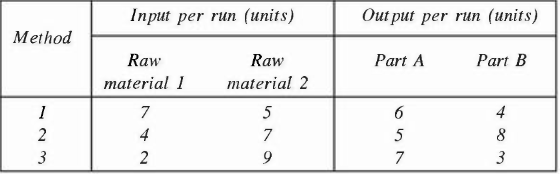
\includegraphics[scale=0.5]{example_production-planning_gupta}
  \scalebox{0.7}{%
    \begin{tabular}{ccccc}
      \toprule
  &\multicolumn{2}{c}{Entrada Por Corrida (unidades)}&\multicolumn{2}{c}{Salidas Por Corrida (unidades)}\\
  \cmidrule{2-5}
  Método&Materia & Materia & Parte&Parte \\
        &prima 1& prima 2&A&B\\
  \midrule
  1&7 &5 &6& 4\\
  2&4&7&5&8\\
  3&2&9&7&3\\
  \bottomrule
\end{tabular}
  } % \scalebox
\par}
\end{frameExample}

\begin{frameExample}{Planeación de la Producción}{}
  La función objetivo a maximizar es  \[ Z = \min \left(  \frac{6x_1 + 5x_2 + 7x_3}{5}, \frac{4x_1 + 8x_2 + 3x_3}{4}\right ) \]
  Las restricciones de disponibilidad de materias primas son:
  \begin{flalign*}
    7x_1 + 4x_2 +2x_3 &\leq 120\\
    5x_1 + 7x_2 +9x_3 &\leq 240\\
  \end{flalign*}
  La formulación anterior viola las propiedades de un programa lineal porque el objetivo es una función no lineal. El modelo se puede transformar a su versión equivalente lineal de la siguiente manera. 
  \[ y =  \min \left(  \frac{6x_1 + 5x_2 + 7x_3}{5}, \frac{4x_1 + 8x_2 + 3x_3}{4}\right )\]
  
\end{frameExample}

\begin{frameExample}{Planeación de la Producción}{}
  Tenemos entonces que
  \begin{flalign*}
    \frac{6x_1 + 5x_2 + 7x_3}{5} & \geq y\\
    \frac{4x_1 + 8x_2 + 3x_3}{4} & \geq y
  \end{flalign*}

  Por lo que el modelo matemático es:
\[ \max Z = y \]
sujeto a (s.t.)
  \begin{columns}[t]
    \column{0.4\textwidth}
\begin{flalign*}
    7x_1 + 4x_2 + 2x_3 & \leq 120\\
    5x_1 + 7x_2 + 9x_3 & \leq 240\\
  \end{flalign*}
  \column{0.4\textwidth}
    \begin{flalign*}
    6x_1 + 5x_2 + 7x_3 - 5y & \geq 0\\
    4x_1 + 8x_2 + 3x_3 - 4y & \geq 0\\
  \end{flalign*}
  \end{columns}
$x_1, x_2, x_3, y   \geq 0 $
\end{frameExample}
%%% Local Variables:
%%% mode: latex
%%% TeX-master: "../slides"
%%% End:

\begin{frameExample}{10. Fluid Blending Problem}{}
  An oil cmpany produces tow grades of gasoline P and Q which it sells at \$ 30, and \$ 40 per litre. The company can buy four different crude oils withthe following constituents and costs:

  {\centering
    \begin{tabular}{ccccc}
      \toprule
      Crude&\multicolumn{3}{c}{Constituents}& Price / litre\\
      \cmidrule{2-4}
      oil&$A$&$B$&$C$& \$ \\
      \midrule
      1&0.75&0.15&0.10 & 20.00\\
      2&0.20&0.30&0.50&22.50\\
      3&0.70&0.10&0.20&25.00\\
      4&0.40&0.10&0.50&27.50\\
      \bottomrule
    \end{tabular}
    \par}

  Gasoline $P$ must have at least 55 per cent of constituent $A$ and no more than 40 per cent of $C$. Gasoline $Q$ must not have more than 25 per cent of $C$. Determine how the crudes should be used to maximize the profit.
\end{frameExample}


%%% Local Variables:
%%% mode: latex
%%% TeX-master: "../slides_linear-programming-intro"
%%% End:

\begin{frameExample}{Production Planning}{}
  % Example 2.6-11 Gupta ebook
  \only<1>{%
    Una empresa que fabrica enfriadores de aire, en la actualidad, tiene pedidos  para los próximos 6 meses. La empresa puede programar su producción durante los próximos 6 meses para cumplir con los pedidos de forma regular o en horas extra. El tamaño del pedido y los costos de producción durante los próximos seis meses son los siguientes:%
  }

  
  \begin{onlyenv}<1,2>
    {%
    \centering
    \scalebox{0.9}{%
      \begin{tabular}{lrrrrrrr}
        \toprule
        &&\multicolumn{6}{c}{Month}\\
        \cmidrule{3-8}
      &&1&2&3&4&5&6\\
      \midrule
      Orders&:&640&660&700&750&550&650\\
      Cost/unit(\$) for&& & & & & & \\
      regular production&:&40&42&41&45&39&40\\
      Cost/unit(\$) for& & & & & & & \\
      overtimeproduction&:&52&50&53&50&45&43\\
      \bottomrule
    \end{tabular}
    }% scalebox
    \par
  }
  \end{onlyenv}
  
  

  \only<2>{%
    Con 100 enfriadores de aire en existencia en la actualidad, la empresa desea tener al menos 150 enfriadores de aire en existencia al final de los 6 meses. La producción regular y extraordinaria en cada mes no debe exceder las 600 y 400 unidades respectivamente. El costo de manejo de inventario para enfriadores de aire es de \$12 por unidad por mes. Formule el modelo de programación lineal (P.L.) para minimizar el costo total.%
  }

  \only<3>{%
    La decisión consiste en determinar el número de unidades de enfriadores que se van a producir en tiempo regular y tiempo extra además de considerar el número de unidades en inventario al final de cada mes.

    Sea $x_{ij}$ el número de unidades fabricadas en el mes $j\, (j = 1, 2, \ldots, 6)$ en tiempo regular o extra $i, (i = 1, 2)$. Además sea $y_j$ el número de unidades en inventario al finalizar el mes $j\, (j = 1, 2, \ldots, 6)$.

    El objetivo es minimizar el costo total (\alert{producir y tener en inventario})
    \begin{flalign*}
      \min Z  =\;\; & 40x_{11} + 42x_{12} + 41x_{13} + 45x_{14} + 39x_{15} + 40x_{16} + \\
      & 52x_{21} + 50x_{22} + 53x_{23} + 50x_{24} + 45x_{25} + 43x_{26} + \\
      & 12(y_{1} + y_{2} + y_{3} + y_{4} + y_{5} + y_{6} )\\
    \end{flalign*}
    % 
    
  }

  \only<4>{%
    Las restricciones son:

    {
      \centering
      \begin{tabular}{rll}
        para el primer mes & $100 + x_{11} + x_{21} - 640$ & $= y_1$\\
        para el segundo mes & $y_1 + x_{12} + x_{22} - 660$ & $= y_2$\\
        para el tercer mes & $y_2 + x_{13} + x_{23} - 700$ & $= y_3$\\
        para el cuarto mes & $y_3 + x_{14} + x_{24} - 750$ & $= y_4$\\
        para el quinto mes & $y_4 + x_{15} + x_{25} - 550$ & $= y_5$\\
        para el sexto mes & $y_5 + x_{16} + x_{26} - 650$ & $= y_6$\\        
      \end{tabular}
      \par}
  }
  \only<5>{%
    \begin{columns}[t]
      \column{0.2\textwidth}
      Restricción de tiempo regular
\begin{align*}
      x_{11} &\leq 600\\
      x_{12} &\leq 600\\
      \vdots &\leq 600\\
      \vdots &\leq 600\\
      x_{16} &\leq 600\\       
    \end{align*}
    \column{0.2\textwidth}
    Restricción de tiempo extra
\begin{align*}
      x_{21} &\leq 400\\
      x_{22} &\leq 400\\
      \vdots &\leq 400\\
      \vdots &\leq 400\\
      x_{26} &\leq 400\\       
\end{align*}
\column{0.2\textwidth}
Condición de no-negatividad
\begin{align*}
  x_{11} &\geq 0\\
  x_{12} &\geq 0\\
  \vdots &\geq 0\\
  \vdots &\geq 0\\
  x_{16} &\geq 0\\
  \end{align*}
  \column{0.2\textwidth}
  Condición de no-negatividad
\begin{align*}
  x_{21} &\geq 0\\
  x_{22} &\geq 0\\
  \vdots &\geq 0\\
  \vdots &\geq 0\\
  x_{26} &\geq 0\\
\end{align*}
\column{0.2\textwidth}
Condición de no-negatividad
\begin{align*}
  y_{1} &\geq 0\\
  y_{2} &\geq 0\\
  \vdots &\geq 0\\
  \vdots &\geq 0\\
  y_{6} &\geq 0\\
  \end{align*}
    \end{columns}    
  }% end only
\end{frameExample}



%%% Local Variables:
%%% mode: latex
%%% TeX-master: "../slides"
%%% End:

\begin{frameExample}{Transportation Problem}{}
  A dairy firm has two milk plants with daily milk production of 6 million litres and 9 million litres respectively. Each day the firm must fulfill the nees of its three distribution centres which have mil requirement of 7, 5 and 3 million litres respectively. Costo of shipping one million litres of milk from each plant to each distribution centre is given, in hundreds of dollars below. Formulate the L.P. model to minimize the transportation cost.

  {
    \centering
   \begin{tabular}{llllrr}
 &  & 1 & 2 & 3 & Supply \\ \cline{3-5}
      & 1 & \multicolumn{1}{|l|}{2} & \multicolumn{1}{l|}{3} & \multicolumn{1}{r|}{11} & 6 \\ \cline{3-5}
     Plants & 2 & \multicolumn{1}{|l|}{1} & \multicolumn{1}{l|}{9} & \multicolumn{1}{r|}{6} & 9 \\ \cline{3-5}
Demand &  & 7 & 5 & 3 & 
\end{tabular}
    \par
  }
\end{frameExample}


%%% Local Variables:
%%% mode: latex
%%% TeX-master: "../slides_linear-programming-intro"
%%% End:

\begin{frameExample}{Product Mix Problem}{}
  A plant manufactures washing machines and dryers. The major manufacturing departments are the stamping deptt., motor and transmission deptt., and assenbly deptt. THe first two departments produce parts ofr both the products while the assembly lines are different for the two products. The monthly deptt. capacities are

  {
    \centering
    \begin{tabular}{rll}
      Stamping deptt. &:& 1,000 washers aor 1,000 dryers\\
      Motor and transmission deptt. &:& 1,600 washers or 7,000 dryers\\
      Washer assembly line &:& 9,000 washers only\\
      Dryer assembly line &:& 5,000 dryers only
    \end{tabular}
    \par
  }

  Profits per piece of washers and dryers are \$ 270 and \$ 300 respectively. Formulate the L.P. model.
\end{frameExample}




%%% Local Variables:
%%% mode: latex
%%% TeX-master: "../slides_linear-programming-intro"
%%% End:

\begin{frameExample}{14. Product Mix Problem}{}
  \begin{onlyenv}<1>
    A certain farming organization operates three farms of comparable productivity. The output of each farm is limited both by the usable acreage and by the amount of water available for irrigation. Following are the data for the upcoming season

  {\centering
    \scalebox{0.8}{%
\begin{tabular}{crr}
      \toprule
      Farm&\multicolumn{1}{c}{Usable acreage}&\multicolumn{1}{c}{Water available} \\
          &&\multicolumn{1}{c}{in acre feet} \\
      \midrule
          1&400&1,500 \\
          2&600&2,000 \\
      3&300&900\\
      \bottomrule
    \end{tabular}
    }
  \par}
  The organization is considering three crops for planting which differ primarily in their expected profit per acre and in their consumption of water. Furthermore, the total acreage that can be devoted to each of the crops is limited by the amount of appropriate harvesting equipment available.
\end{onlyenv}

\begin{onlyenv}<2>
  {\centering
    \scalebox{0.8}{%
      \begin{tabular}{cccc}
        \toprule
        Crop & Minimum acreage& Water consumption& Expected profit\\
             & &in acre feet per acre& per acre \$\\
        \midrule
        A&400&5&400\\
        B&300&4&300\\
        C&300&3&100\\
        \bottomrule
      \end{tabular}
    }
    \par}

  In order to maintain a uniform work load among the farms, it is the policy of the organization that the percentage of the usable acreage planted must be the same at each farm. However, any combination of the crops may be grown at any of the farms. The organization wishes to know how much of each crop should be planted at the respective farms in orders to maximize expected profit. Formulate this as a linear programming problem.
\end{onlyenv}
\end{frameExample}


%%% Local Variables:
%%% mode: latex
%%% TeX-master: "../slides_linear-programming-intro"
%%% End:

\begin{frameExample}{Product Mix Problem}{}
  % 2.6-15 Gupta Ebook
  \only<1>{%
    Consider the following problem faced by a production planner in a soft drink plant. He has two bottling machines $A$ and $B$. $A$ is designed for 8-ounce bottles and $B$ for 16-ounce bottles. However; each can be used on both types of Bottles with som loss of efficiency. The following data are available:%
  }

    \begin{onlyenv}<1>
  {\centering
      \begin{tabular}{ccc}
      \toprule
      Machine&8-ounce bottles&16-ounce bottles \\
      \midrule
      $A$&100/minute&40/minute \\
      $B$&60/minute&75/minute\\
      \bottomrule
    \end{tabular}
    \par}
  \end{onlyenv}

  \only<2>{%
  The machines can be run 8-hour per day, 5 days a week. Profit on 8-ounce bottle is 15 paise and on 16-ounce bottle is 25 paise. Weekly production of the drink cannot exceed 300,000 ounces and the market can absorb 25,000 eight-ounce bottles and 7,000 sixteen-ounce bottles per week. The planner wishes to maximize his profit subject, of course, to all the production and marketing constraints. Formulate this as L.P. problem.
  }
\end{frameExample}


%%% Local Variables:
%%% mode: latex
%%% TeX-master: "../slides_linear-programming-intro"
%%% End:

\begin{frameExample}{Product Mix Problem}{}
  \begin{onlyenv}<1>
      A manufacturer of biscuits is considering four ytpes of gift-packs containing three types of biscuits: orange cream(o.c.) chocolate cream (c.c.) and wafers (w.). Market research conducted to assess the preferences of the costumers shows the following types of assortments to be in good demand:

  {
    \centering
    \begin{tabular}{clc}
      \toprule
      Assortment    & Contents&	Selling price/kg \$\\
      \midrule
A&	Not less than 40 \% of o.c.&	200\\
&	Not more than 20\% of c.c.&	\\
B&	Not less than 20\% of o.c.&	250\\
&	Not more than 40\% of c.c.&	\\
C&	Not less than 50\% of o.c.&	220\\
&	Not more than 10\% of c.c.&	\\
      D&	No restrictions	&120\\
      \bottomrule
    \end{tabular}
    \par
  }
\end{onlyenv}

\begin{onlyenv}<2>
  For the biscuits the manufacturing capacity and costs are given below.
  
  {
    \centering
    \begin{tabular}{ccc}
      \toprule
      Biscuit variety&	Plant capacity&	Manufacturing cost\\
                     &(kg / day)&	(\$ / kg)\\
      \midrule
      o.c.&	200&	80\\
      c.c.	&200&	90\\
      w.	&150&	70\\
      \toprule
    \end{tabular}
    \par
  }

  Formulate the L.P. model to finde the production schedule to find the production schedule which maximizes the profit assuming that there are no market restrictions.
\end{onlyenv}
\end{frameExample}


%%% Local Variables:
%%% mode: latex
%%% TeX-master: "../slides_linear-programming-intro"
%%% End:

\begin{frameExample}{Product Mix Problem}{}
  % Example Gupta 2.6-17
  A manufacturer has five lathes and three milling machines in his workshop and produces and assembly that consists of 2 units of part A and 3 units of part B. The processing time for each part on the two types of machines is given below.

  {
    \centering
    \scalebox{0.9}{%
      \begin{tabular}{ccc}
        \toprule
        Part&\multicolumn{2}{c}{Processing time in minutes on a} \\
        \cmidrule{2-3}
            &Lathe&Milling machine \\
        \midrule
        A&10&18 \\
        B&25&12\\
        \toprule
      \end{tabular}
    }
    \par
  }

  In order to maintain a uniform work-load on the two types of machines, the manufacturer has framed a policy that no type of machine should run more than 40 minutes per day longer than the other machine. Formulate the L.P. problem if the objective is to produce the maximum number of assemblies in any 8-hour working day.
\end{frameExample}


%%% Local Variables:
%%% mode: latex
%%% TeX-master: "../slides_linear-programming-intro"
%%% End:

\begin{frameExample}{}{}
    % example-2.6-18
  \only<1>{%
A firm produces three different products, 1, 2 and 3. Each product needs
to be processed through two departments, $A$ and $B$. Department
$A$ has two machines $A_1$ and $A_2$, while $B$ has three
machines, $B_1$, $B_2$ and $B_3$. Product 1 can be manufactured on
any type of $A$ and $B$ machines. Product 2 can be manufactured on
any of type $A$ machines and only on $B_1$ of type $B$ machines.
Product 3 can be manufactured on machines $A_2$ of type $A$ and
$B_3$ of type $B$. Time taken to manufacture one unit of each of
product on each type of machine is given in table below. The table also
shows total available machine time per week, cost of running each
machine at full capacity in a week, cost of raw material required per
unit product and sale price per unit product. How many of each type of
product be manufactured on which machine so as to maximize the net
profit ? Formulate the L.P. model for the problem.
  }

  \begin{onlyenv}<2>
    {\centering
  \scalebox{0.7}{
    \begin{tabular}{llllll}
\toprule
Machine & 1 & 2 & 3 & Time per week (minutes) & Cost / week at full
capacity \\
\midrule
$A_1$ & 4 & 5 & -- & 5,000 & 250 \\
$A_2$ & 5 & 7 & 11 & 10,000 & 500 \\
$B_1$ & 7 & 8 & -- & 8,000 & 450 \\
$B_2$ & 8 & -- & -- & 4,000 & 250 \\
$B_3$ & 3 & -- & 7 & 5,600 & 280 \\
Material Cost & 0.30 & 0.40 & 0.50 & & \\
Sale price & 1.50 & 1.80 & 2.40 & & \\
\bottomrule
\end{tabular}
} % end scale box
\par}
  \end{onlyenv}

\end{frameExample}


\section{Activities}
\label{sec:activities}


\begin{frameact}{Riser Sports Products}{}
  % Anderson 07-22
  Reiser Sports Products quiere determinar la cantidad de balones de futbol de All-Pro (A)
y Universitario (U) a producir con el fin de maximizar las utilidades durante el siguiente horizonte de planeación de cuatro semanas. Las restricciones que afectan las cantidades de
producción son las capacidades de producción en tres departamentos: corte y teñido, costura
e inspección y empaque. Para el periodo de planeación de cuatro semanas se dispone de 340 horas de corte y teñido, 420 horas de costura y 200 horas de inspección y empaque. Los tiempos requeridos para elaborar un balón A y U en el departamento de corte y teñido son de 12 y 6 horas respectivamente. El departamento de costura requiere 9 horas para un balón A y 6 horas para elaborar un balón U. En la inspección se ocupan 6 horas para cada balón de fútbol. Los balones de futbol All-Pro producen utilidades de \$5 por unidad y los balones Universitarios producen una utilidad de \$4 por unidad. Formule un modelo para el problema.
\end{frameact}



%%% Local Variables:
%%% mode: latex
%%% TeX-master: "../slides"
%%% End:

\begin{frameact}{Reddy Mikks }

\label{example:reddy-mikks}
  % Ejemplo 2.1-1 (La compañía Reddy Mikks) Taha
  \only<1>{%
    Reddy Mikks produce pinturas para interiores y exteriores con dos materias primas, $M_1$ y $M_2$. La tabla siguiente proporciona los datos básicos del problema. Una encuesta de mercado indica que la demanda diaria de pintura para interiores no puede exceder la de pintura para exteriores en más de una tonelada. Asimismo, que la demanda diaria máxima de pintura para interiores es de dos toneladas. Reddy Mikks se propone determinar la (mejor) combinación óptima de pinturas para interiores y exteriores que maximice la utilidad diaria total.%
  }


  {\centering
  \includegraphics<1>[scale=0.6]{reddy-mikks_01}
  \par}
\end{frameact}






%%% Local Variables:
%%% mode: latex
%%% TeX-master: "../slides_linear-programming-intro"
%%% End:

\begin{frameact}{}{}
  % Taha 02-02A-04
\label{act:taha_02-02A-04}
  Una compañía que funciona 10 horas al día fabrica dos productos en tres procesos secuenciales. La siguiente tabla resume los datos del problema:

  {
    \centering
    \begin{tabular}{ccccc}
      \toprule
      &\multicolumn{3}{c}{Minutos por unidad}&Utilidad\\
      \cmidrule{2-4}
      Producto& Proceso 1& Proceso 2& Proceso 3& Unitaria (\$)\\
      \midrule
1&10&6&8&2\\
      2&5&20&10&3\\
      \bottomrule
    \end{tabular}
    \par
  }
  
  Determine la combinación óptima de los dos productos.
\end{frameact}


%%% Local Variables:
%%% mode: latex
%%% TeX-master: "../slides_linear-programming-intro"
%%% End:

\begin{frameact}{}{}
  % Taha 02-02A-05
\label{act:taha_02-02A-05}
  Una compañía fabrica dos productos, A y B. El volumen de ventas de A es por lo menos 80\% de las ventas totales de A y B. Sin embargo, la compañía no puede vender más de 100 unidades de A por día. Ambos productos utilizan una materia prima, cuya disponibilidad diaria máxima es de 240 lb. Las tasas de consumo de la materia prima son de 2 lb por unidad de A y de 4 lb por unidad de B. Las utilidades de A y B son de \$20 y \$50, respectivamente. Determine la combinación óptima de productos para la compañía.

  \only<2>{
  \begin{columns}[t]
      \column{0.5\textwidth}
      Modelo simplificado
      
      \[\max Z = 20x_1 + 50x_2\]

\begin{align}
0.20x_1 - 0.80x_2 &\geq 0\\
x_1 &\leq 100\\
2x_1 + 4x_2&\leq 240\\[3mm]
x_1, x_2&\geq 0
\end{align}
%
\column{0.5\textwidth}
Modelo en forma canónica
\[\max Z = 20x_1 + 50x_2\]

\begin{align}
-0.20x_1 + 0.80x_2 &\leq 0\\
x_1 &\leq 100\\
2x_1 + 4x_2&\leq 240\\[3mm]
x_1, x_2&\geq 0
\end{align}
  \end{columns}
  } % end only
\end{frameact}


%%% Local Variables:
%%% mode: latex
%%% TeX-master: "../slides"
%%% End:

\question
  % Taha 02-02A-06
  \label{act:taha_02-02A-06}
  Alumco fabrica láminas y varillas de aluminio. La capacidad de producción máxima se estima en 800 láminas o 600 varillas por día. La demanda diaria es de 550 láminas y 580 varillas. La utilidad por tonelada es de \$40 por lámina y de \$35 por varilla. Determine la
combinación de producción diaria óptima.


\begin{solution}

  {\centering
    $\max Z = 40x_1 + 35x_2$
    
      \begin{align*}
        \frac{x_1}{800} + \frac{x_2}{600} &\leq 1\\
        x_1 &\leq 550\\
        x_2 &\leq 580
      \end{align*}

    $x_1, x_2 \geq 0$
  \par}
\end{solution}


%%% Local Variables:
%%% mode: latex
%%% TeX-master: "activities"
%%% End:


\section{Programming Examples}
\label{sec:programming}

\begin{framecode}{}{}
  \lstinputlisting{scripts/example02-01.py}
\end{framecode}
\begin{framecode}{}{}
  \lstinputlisting{scripts/example02-02.py}
\end{framecode}
\begin{framecode}{}{}
  \lstinputlisting{scripts/example02-03.py}
\end{framecode}
\begin{frame}
  \maketitle
\end{frame}


\end{document}
